\documentclass{beamer}
\usetheme{Montpellier}
\usepackage{german}

\usepackage[utf8x]{inputenc}

\usepackage{amssymb}
\usepackage{amsmath}

\usepackage{braket}

\usepackage{listings}
\usepackage{color}

\definecolor{sourcecodered}{rgb}{0.6,0,0} % for strings
\definecolor{sourcecodegreen}{rgb}{0.25,0.5,0.35} % comments
\definecolor{sourcecodepurple}{rgb}{0.5,0,0.35} % keywords
\definecolor{sourcecodedocblue}{rgb}{0.25,0.35,0.75} % javadoc

\lstset{
	language=C,                                    % the language of the code
	basicstyle=\ttfamily\small,                    % the size of the fonts that are used for the code
	keywordstyle=\ttfamily\small,                  % keyword style
	stringstyle=\ttfamily\small,                   % string literal style
	commentstyle=\ttfamily\small,                  % comment style
	numbers=none,                                  % where to put the line-numbers; possible values are (none, left, right)
	numberstyle=\small\color{black},               % the style that is used for the line-numbers
	numbersep=6pt,                                 % how far the line-numbers are from the code
	tabsize=4,	                   	               % sets default tabsize to 4 spaces
	showspaces=false,                              % show spaces everywhere adding particular underscores; it overrides 'showstringspaces'
	showstringspaces=false,                        % underline spaces within strings only
	showtabs=false,                                % show tabs within strings adding particular underscores
	%	title=\lstname,                                % show the filename of files included with \lstinputlisting; also try caption instead of title
	breaklines=true,                               % sets automatic line breaking
	breakatwhitespace=true,                             % sets if automatic breaks should only happen at whitespace
	frame=single,	                                     % adds a frame around the code
	rulecolor=\color{black},                             % if not set, the frame-color may be changed on line-breaks within not-black text (e.g. comments (green here))
	literate=%
	{Ö}{{\"O}}1
	{Ä}{{\"A}}1
	{Ü}{{\"U}}1
	{ß}{{\ss}}1
	{ü}{{\"u}}1
	{ä}{{\"a}}1
	{ö}{{\"o}}1
	{~}{{\textasciitilde}}1
	% backgroundcolor=\color{white},      % choose the background color; you must add \usepackage{color} or \usepackage{xcolor}; should come as last argument
	% captionpos=b,                       % sets the caption-position to bottom
	% deletekeywords={...},               % if you want to delete keywords from the given language
	% escapeinside={\%*}{*)},             % if you want to add LaTeX within your code
	% extendedchars=true,                 % lets you use non-ASCII characters; for 8-bits encodings only, does not work with UTF-8
	% keepspaces=true,                    % keeps spaces in text, useful for keeping indentation of code (possibly needs columns=flexible)
	% morekeywords={*,...},               % if you want to add more keywords to the set
	% stepnumber=2,                       % the step between two line-numbers. If it's 1, each line will be numbered
}

\begin{document}
	\title{Git \& Github Tutorial}   
	\author{Daniel Schädler \& Jean-Pierre Hotz} 
	\date{22. October 2018}
	%\logo{\includegraphics[scale=0.14]{logo-SF}}
	
	\subtitle{} %Untertitel
	\institute[DHBW KA]{DHBW Karlsruhe}%Angabe des Institutes
	%\logo{\pgfimage[width=2cm,height=2cm]{bnslogo}}%Die Datei hulogo.pdf (bzw. hulogo.png, hulogo.jpg, hulogo.mps bei Verwendung von pdftex als Backend) als Logo auf allen Folien, hier mithilfe des Paketes pgf.
	%\titlegraphic{\includegraphics[width=2cm,height=2cm]{bnslogo}}%Die Datei hulogo.pdf (bzw. analog wie bei \logo auch entsprechendes Format) als Logo nur auf der Titelseite unter Verwendung des Paketes graphicx.
	\subject{Software-Engineering}%Setzt Thema in den PDF-Dokument-Eigenschaften
	\keywords{}%Setzt Schlüsselwörter in den PDF-Dokument-Eigenschaften
	
	\setbeamertemplate{navigation symbols}[vertical]
	
	\begin{frame}
		\titlepage
	\end{frame}
	
	\begin{frame}
		\tableofcontents
	\end{frame}

	\section{General}
	\begin{frame}
		\frametitle{General}\pause
		\begin{itemize}
			\item Git is a \textbf{V}ersion \textbf{C}ontrol \textbf{S}ystem \pause
			\item created in 2005 by Linus Torvalds
		\end{itemize}
	\end{frame}

	\section{Terminology}
	\begin{frame}
		\frametitle{Terminology}\pause
		\begin{itemize}
			\item Commit (History) \pause
			\item Branch (Merge) \pause
			\item (Remote) Repository
		\end{itemize}
	\end{frame}

	\section{Git areas}
	\begin{frame}
		\frametitle{Git areas}
		\begin{figure}[h]
			\centering
			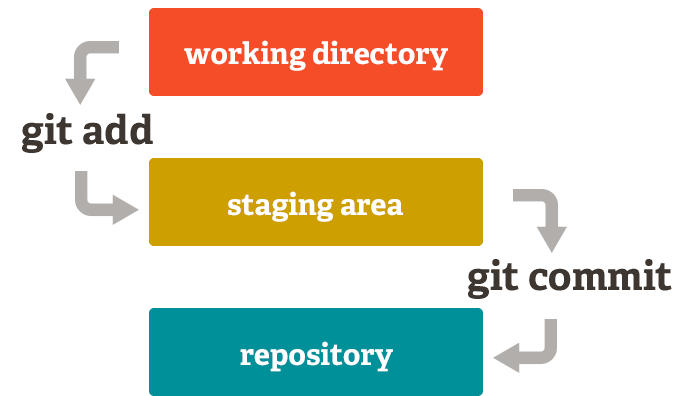
\includegraphics[width=.9\linewidth]{git-areas.png}
			\label{fig1}
		\end{figure}
	\end{frame}

	\begin{frame}
		\frametitle{Git areas}\pause
		\begin{itemize}
			\item exclude files with \lstinline|.gitignore|-file \pause
			\item contains patterns \pause
			\item \lstinline|*| matches anything \pause
			\item postceding \lstinline|/| matches a folder \pause
			\item preceding \lstinline|/| matches only in the root folder \pause
			\item preceding \lstinline|!| negates the pattern (i.e. includes files)
		\end{itemize}
	\end{frame}

	\begin{frame}[fragile]
		\centering What do the following rules exclude?
		\begin{lstlisting}
/src/
!/src/working/
		\end{lstlisting}
	\end{frame}

	\section{Local repositories}
	\begin{frame}
		\frametitle{Local repositories}\pause
		\begin{itemize}
			\item create new local repository (\lstinline|git init|) \pause
			\item clone a remote repository (\lstinline|git clone <URL>|)
		\end{itemize}
	\end{frame}

\end{document}